%% Adaptado a partir de :
%%    abtex2-modelo-trabalho-academico.tex, v-1.9.2 laurocesar
%% para ser um modelo para os trabalhos no IFSP-SPO

\documentclass[
    % -- opções da classe memoir --
    12pt,               % tamanho da fonte
    openright,          % capítulos começam em pág ímpar (insere página vazia caso preciso)
    %twoside,            % para impressão em verso e anverso. Oposto a oneside
    oneside,
    a4paper,            % tamanho do papel. 
    % -- opções da classe abntex2 --schwinn
    % Opções que não devem ser utilizadas na versão final do documento
    %draft,              % para compilar mais rápido, remover na versão final
    paginasA3,  % indica que vai utilizar paginas em A3 
    MODELO,             % indica que é um documento modelo então precisa dos geradores de texto
    TODO,               % indica que deve apresentar lista de pendencias 
    % -- opções do pacote babel --
    english,            % idioma adicional para hifenização
    brazil              % o último idioma é o principal do documento
    ]{ifsp-spo-inf-ctds} % ajustar de acordo com o modelo desejado para o curso



% ---
% Informações de dados para CAPA e FOLHA DE ROSTO
% ---
\titulo{Lixt}

% Trabalho individual
%\autor{AUTOR DO TRABALHO}

% Trabalho em Equipe
% ver também https://github.com/abntex/abntex2/wiki/FAQ#como-adicionar-mais-de-um-autor-ao-meu-projeto
\renewcommand{\imprimirautor}{
\begin{tabular}{lr}
Alkindar José Ferraz Rodrigues & SP3029956 \\
Carolina de Moraes Josephik & SP3030571 \\
Fabio Mendes Torres & SP3023184 \\
Gabriely de Jesus Santos Bicigo & SP303061X \\
Leonardo Naoki Narita & SP3022498 \\
Mariana da Silva Zangrossi & SP3030679 \\
\end{tabular}
}


\disciplina{PI1 - Projeto Integrado I}

\preambulo{Desenho de aplicação para desenvolvimento
na disciplina de Projeto Integrado I no 1°
semestre de 2021.}

\data{Junho de 2021}

% Definir o que for necessário e comentar o que não for necessário
% Utilizar o Nome Completo, abntex tem orientador e coorientador
% então vão ser utilizados na definição de professor
\renewcommand{\orientadorname}{Professor:}
\orientador{Ivan Francolin Martinez}
\renewcommand{\coorientadorname}{Professor:}
\coorientador{José Braz de Araujo}


% ---


% informações do PDF
\makeatletter
\hypersetup{
        %pagebackref=true,
        pdftitle={\@title}, 
        pdfauthor={\@author},
        pdfsubject={\imprimirpreambulo},
        pdfcreator={LaTeX with abnTeX2 using IFSP model},
        pdfkeywords={abnt}{latex}{abntex}{abntex2}{IFSP}{\ifspprefixo}{trabalho acadêmico}, 
        colorlinks=true,            % false: boxed links; true: colored links
        linkcolor=blue,             % color of internal links
        citecolor=blue,             % color of links to bibliography
        filecolor=magenta,              % color of file links
        urlcolor=blue,
        bookmarksdepth=4
}
\makeatother
% --- 

\graphicspath{ {./images} }
\usepackage{float}

% carregando aqui referencias quando utilizando BIBLATEX
\IfPackageLoaded{biblatex}{%
\addbibresource{referencias.bib}
\addbibresource{exemplos/abntex2-doc-abnt-6023.bib}
}{}

% ----
% Início do documento
% ----
\begin{document}


% Retira espaço extra obsoleto entre as frases.
\frenchspacing 

\newpage

% ----------------------------------------------------------
% ELEMENTOS PRÉ-TEXTUAIS
% ----------------------------------------------------------
\pretextual

% ---
% Capa
% ---
\imprimircapa

\newcounter{todocounter}
\newcommand{\todonum}[2][]
{\stepcounter{todocounter}\todo[#1]{\thetodocounter: #2}}

% ---
% Folha de rosto
% (o * indica que haverá a ficha bibliográfica)
% ---
\imprimirfolhaderosto
%\imprimirfolhaderosto*
% ---

% -- resumo obrigatório
% ---
% RESUMOS
% ---

% resumo em português
\setlength{\absparsep}{18pt} % ajusta o espaçamento dos parágrafos do resumo
\begin{resumo}

O presente documento tem como objetivo apresentar o desenho do projeto Lixt, solução tecnólogica
que visa facilitar a gestão de controle de gastos em mercado e gerenciamento das listas de compras individuais ou colaborativas. 
A plataforma dá autonomia para o usuário gerir listas, membros de uma lista, produtos, categorias dos produtos e compras. O Lixt ainda se propõe a oferecer a análise das compras realizadas e fornecer o histórico de compras para que o usuário consiga obter melhor controle sobre suas despesas de mercado. 
Para implementação da proposta utilizamos o banco de dados MySQL com back-end construído em Java aliado ao Spring e ao Hibernate. Na implementação mobile utilizamos Javascript com o framework React-Native. A hospedagem dos recursos
ficará na plataforma Amazon Web Services. Para gerenciarmos a equipe durante o projeto optamos pela utilização do scrum e do kanban. 

 \textbf{Palavras-chaves}: lista de compras. compras. organização financeira.
\end{resumo}

% resumo em inglês
\begin{resumo}[Abstract]
 \begin{otherlanguage*}{english}
This document aims to present the design of the Lixt project, a technological solution that aims to facilitate the management of expenses control in groceries and management of individual or collaborative shopping lists.
The platform eanbles the user to manage lists, list members, products, product categories and purchases. Lixt also proposes to offer an analysis of the purchases made and provide the purchase history so that the user can obtain better control over their groceries expenses.
To implement the proposal, we decided to use the MySQL database and to develop the back-end in Java together with Spring and Hibernate. In the mobile implementation it uses Javascript with the React-Native framework. We chose to host the resources on the Amazon Web Services platform. To manage the team during the project, we chose to use scrum and kanban.
   \vspace{\onelineskip}

   \noindent 
   \textbf{Keywords}: shopping list. groceries. financial organization.
 \end{otherlanguage*}
\end{resumo}


% ---
% inserir lista de ilustrações
% ---
\pdfbookmark[0]{\listfigurename}{lof}
\listoffigures*
\cleardoublepage
% ---

% ---
% inserir lista de tabelas
% ---
%\pdfbookmark[0]{\listtablename}{lot}
%\listoftables*
%\cleardoublepage
% ---

% ---
% inserir lista de quadros
% ---
\pdfbookmark[0]{\listofquadrosname}{loq}
\listofquadros*
\cleardoublepage
% ---

% ---
% inserir lista de abreviaturas e siglas
% ATENCAO o SHARELATEX/OVERLEAF GERA O GLOSSARIO SOMENTE UMA VEZ
% CASO SEJA FEITA ALGUMA ALTERAÇÃO NA LISTA DE SIGLAS É NECESSARIO UTILIZAR A OPÇÃO :
% "Clear Cached Files" DISPONIVEL NA VISUALIZAÇÃO DOS LOGS 
% ---
% https://www.sharelatex.com/learn/Glossaries


\ifdef{\printnoidxglossary}{
    \printnoidxglossary[type=\acronymtype,title=Lista de abreviaturas e siglas,style=siglas]
    \cleardoublepage
}{}





% ---
% inserir o sumario
% ---
\pdfbookmark[0]{\contentsname}{toc}
\tableofcontents*
\cleardoublepage
% ---


% ----------------------------------------------------------
% ELEMENTOS TEXTUAIS
% ----------------------------------------------------------
\textual

\chapter{Introdução}

\label{sec:contextualizao}
\section{Contextualização}
Ir às compras é uma atividade essencial no cotidiano das pessoas. Tanto por uma questão de sobrevivência, envolvendo compra de alimentos, medicamentos, produtos de higiene pessoal e da casa, quanto por uma questão de lazer.

Quando se trata de compras essenciais, ou seja, aquelas nas quais os produtos adquiridos tem o papel de reabastecer funções de necessidades básicas, as compras de varejo alimentar não podem ser desconsideradas, devido sua importância e frequência. Conforme a pesquisa “Tendências e Comportamento do Consumidor” \cite{APAS}, realizada em 2018 pela Associação Paulista de Supermercados (APAS), 89\% da população com 16 anos ou mais costuma ir ao supermercado mesmo que ocasionalmente. Um consumidor, em média, faz quatro visitas ao supermercado por mês e um em cada três frequentadores costuma ir ao supermercado pelo menos uma vez por semana. Além disso, os supermercados foram apontados como o estabelecimento favorito de varejo alimentar por 53\% dos participantes, seguido pelo hipermercado, com 13\%.

Para melhor entendimento dos resultados apresentados e que serão apresentados ao decorrer do documento, é necessária a definição das diversas categorias de estabelecimentos de compra de varejo alimentar com o formato autosserviço, que se refere à estabelecimentos em que o consumidor compra o produto sem a necessidade de haver a intermediação de um funcionário da loja, antes de realizar o \textit{check-out}. Esses estabelecimentos podem ser categorizados como:
\begin{itemize}
\item Supermercado: Se refere à loja alimentar caracterizada pela disposição de produtos no formato autosserviço, separados por quatro áreas básicas (perecíveis, mercearia, limpeza doméstica e bebidas) e pela existência de pelo menos dois \textit{check-outs} na saída. Possui de 1.500 a 5.000 itens disponíveis.
\item Hipermercado: Se refere à loja alimentar do tipo autosserviço, que oferece vendas de mercearia, bazar, perecíveis, têxteis e eletrodomésticos. Possuem mais de 5.000 itens em exposição e mais de 40 \textit{check-outs} espalhados no estabelecimento.
\item Lojas com apenas 1 \textit{check-out}: Pequenas lojas de varejo alimentar, como mercearias, lojas de bairro e conveniência. Apesar que, no caso das lojas de conveniência, pode ser encontrados estabelecimentos com até três \textit{check-outs}.
\end{itemize}

Além de estabelecimentos de varejo alimentar com o formato autosserviço, também são encontradas lojas do setor de hortifrúti, como feiras livres e lojas de bairro focadas exclusivamente nesse tipo de alimento. Essas lojas podem ser chamadas de mercados independentes, pois são operadas por empresas que possuem até 4 lojas que operam sobre a mesma marca. De forma contrária, uma rede de mercados ou supermercados é formada por no mínimo 5 lojas que operam sobre a mesma marca.

Entretanto, alguns hábitos de consumo foram modificados devido à pandemia da COVID-19, declarada nos primeiros meses de 2020. O isolamento social, considerado uma importante medida de prevenção ao coronavírus no Brasil e no restante do mundo, fez com que os consumidores brasileiros realizassem menos visitas aos estabelecimentos de varejo alimentar, mas levado cada vez mais produtos para casa, segundo o levantamento de dados realizado pela Dotz \cite{Dotz}. Outra pesquisa, realizada pela Asserj \cite{Asserj}, apontou que 84\% dos entrevistados vão ao supermercado apenas uma vez por mês, enquanto 10\% fazem compras duas vezes por mês e 6\% restante afirma fazer compras semanalmente. Os dados mostrados refletem a mudança de hábito dos consumidores, que antes compravam gradualmente, ao longo do mês, mas que agora, passou a concentrar as compras tudo em um único dia, em busca de evitar exposição ao coronavírus, e economizar.

Além da mudança de hábitos relacionados à frequência e quantidade de produtos em cada compra, as compras de produtos básicos para cozinhar em casa cresceram, e a busca por compras em supermercados, hipermercados e atacarejos também, de modo a criar estoques de alimentos nas casas, segundo pesquisa realizada pela Nielsen Brasil \cite{NielsenBrasil}.

De certa maneira, pode-se dizer que, independente das condições externas, as compras em estabelecimentos de varejo alimentar são muito presentes no cotidiano das famílias brasileiras. Por isso, devem ter sua devida atenção e gerenciamento, principalmente por questões financeiras, e de organização, a fim de alcançar o objetivo de comprar mais produtos de maior qualidade gastando menos.

\label{sec:problematizacao}
\section{Problematização}
Por ser algo tão presente na vida de todas as famílias do país, independentemente da frequência das visitas aos estabelecimentos e a quantidade de produtos nos quais são comprados, a falta de planejamento no momento de realizar uma nova compra pode acarretar problemas financeiros.

Em uma pesquisa realizada em 2015 pela empresa Serviço de Proteção ao Crédito (SPC Brasil) \cite{SPC}, foi apontado que 33\% das compras feitas por impulso são de supermercado ou estabelecimentos de varejo alimentar. As razões principais que os participantes da pesquisa compartilharam foram em relação ao produto estar mais barato, devido a uma promoção, ou por falta de planejamento.

Além das compras por impulso, que geram valores mais altos no \textit{check-out}, outro problema gerado pela falta de planejamento é o destino dos produtos comprados. Segundo o Instituto Akatu \cite{Akatu}, cerca de 30\% das compras de mercado vão para o lixo.

Tendo em vista as consequências que a falta de planejamento nas compras pode gerar, como altos gastos e desperdício de alimentos e dinheiro, é possível concluir que as pessoas não saibam administrar e controlar seus gastos em supermercados, mesmo existindo meios de fazê-lo.

Atualmente, as maneiras tradicionais de um consumidor de fazer pesquisas de preço e controlar seus gastos é através dos panfletos oferecidos pelos estabelecimentos, nos quais mostram ofertas e descontos, e através do cupom fiscal. De acordo com a Pesquisa Tendências do Consumidor de 2018 \cite{PesquisaAPAS}, 69\% dos participantes declararam que realizam pesquisas de preço antes de comprarem determinado produto, através das seguintes formas:
\begin{itemize}
\item Indo ao supermercado (59\%).
\item Consultando ofertas em jornais e folhetos (50\%).
\item Buscas na Internet (12\%).
\end{itemize}

No momento de controlar os gastos e administrá-los de maneira detalhista, a única forma é através do cupom fiscal, um documento frágil que contém todos os produtos comprados e seus respectivos preços, além dos impostos cobrados, data e hora da compra e o nome do estabelecimento. Sua fragilidade é devido a sua composição, o que ocasiona o desaparecimento das informações ao decorrer do tempo. Ao depender do cupom fiscal para analisar e atualizar os gastos, ocorrem alguns dos seguintes problemas:
\begin{itemize}
\item Só é possível fazer uma análise de gastos após a compra, sendo que o consumidor teria grandes benefícios ao analisar os gastos e produtos durante a compra.
\item Dificuldade de lembrar e guardar os preços dos alimentos e produtos durante a compra, para futura análise que auxilie o comprador a fazer compras mais econômicas e de qualidade.
\item É necessário repassar manualmente todos os dados de cada cupom fiscal para um documento centralizado, caso o consumidor queira manter um histórico de compra ou fazer uma análise geral.
\item Dificuldade em analisar preços de diferentes estabelecimentos de modo a decidir qual o melhor custo-benefício julgado pelo comprador, já que essa informação vai provavelmente constar em algum meio não centralizado, ou seja, o consumidor irá perder a informação rapidamente.
\item Dificuldade em analisar e calcular quais as categorias de produtos que possuem maior gasto, menor gasto, ou uma média, baseados em determinado período, que visa facilitar a descoberta de quais produtos são mais comprados, quais são mais caros, de modo a auxiliar o usuário em futuras compras.
\item Dificuldade de gerenciar compras colaborativas, cada participante não sabe exatamente o que será comprado ou quais itens serão de sua responsabilidade, a não ser que essas informações sejam compartilhadas através de meios que a ação manual seria necessária, como mandar uma mensagem através de um aplicativo.
\end{itemize}

\label{sec:justificativa}
\section{Justificativa}
Para o total controle e gerenciamento das compras, seria necessário utilizar métodos para a pesquisa de preço, e a análise do cupom fiscal. Apesar de ser possível utilizar a busca na Internet para realizar a pesquisa de preço, essa forma é pouco utilizada entre as pessoas, além de as informações não serem centralizadas, ocasionando na demora para realizar a pesquisa. Além disso, ambos métodos são manuais, e não há muitas possibilidades de automatizá-los. A falta de automatização gera maior dificuldade para as pessoas realizarem seus planejamentos, o que acaba ocasionando em gastos cada vez mais altos em cada compra realizada, sendo cada vez mais difícil de entender e analisar os motivos que fazem o bolso ficar mais pesado no final do mês.

O agravamento dos problemas financeiros podem trazer consequências graves, fora ser um tópico presente nas famílias brasileiras. Conforme estudos realizados pela SPC Brasil em 2020, foi revelado que a meta principal do brasileiro é guardar dinheiro \cite{MetaFinanceiraSPC}, e que apenas 1 a cada 10 brasileiros tem renda suficiente para pagar as despesas de início de ano \cite{DespesaSPC}. Além do mais, problemas financeiros podem gerar problemas psicológicos e de saúde, como foi levantado pelo estudo realizado pela The Employer’s Guide to Financial Wellness 2019 \cite{Endividados}, que apontam que pessoas endividadas têm 4 vezes mais chances de desenvolver depressão, e 8 vezes mais chances de desenvolver insônia.

Considerando os problemas citados acima, o gerenciamento e administração de compras é extremamente essencial no contexto vivido por tantos brasileiros, tanto por uma questão financeira, de administrar as contas, sobreviver, e construir sonhos, como também de saúde.

\label{sec:objetivos}
\section{Objetivos}
Para solucionar todos os problemas citados e no que eles acarretam, entregando autonomia, controle de compras para os consumidores de maneira intuitiva e fácil, em que todas as informações que eles registrem sejam armazenadas em um local centralizado, criamos o Lixt, uma solução que facilite a vida do consumidor que reside no Brasil, para o gerenciamento e controle de suas compras através de criação e edição de listas de compras compartilhadas ou individuais. A solução será focada em facilitar as compras alimentícias, feitas em supermercados, feiras, lojas de conveniência, e até mesmo em aplicativos de alimentos, como IFood, Uber Eats, Rappi, e entre outros.

Além disso, o Lixt se propõe em oferecer análises de compras por determinado período escolhido pelo usuário, separar produtos em categorias e até mesmo apresentar análises quanto a variação de preço entre estabelecimentos, que poderão ser adicionados de acordo com a preferência do usuário, além de outras funcionalidades que estarão melhores descritas na seção de Escopo. Dessa maneira, o planejamento de compras alimentares torna-se automatizada e substituí formas manuais de gerenciamento de gastos.

\label{sec:analiseconcorrencia}
\section{Análise da Concorrência}
Auditamos soluções que existem atualmente no mercado e, ao verificar as aplicações existentes, conclui-se que há intersecções nas funções dentre os aplicativos analisados. As funções mais básicas, como gerenciamento de itens e gerenciamento de listas, estão presentes em todos, tendo em vista que são essenciais em qualquer aplicativo de
lista. Outras funções básicas que deveriam ser incluídas em qualquer aplicação de lista, como gerenciamento de categorias e
compartilhamento de listas, não estão presentes em todos os
aplicativos analisados.

Contudo, as divergências ficam claras quando analisamos o mecanismo das aplicações, entre elas destacam-se o \textit{Mealime} e o \textit{Cozi Family Organizer} que, apesar de serem voltados para as compras, cumprem também outras funcionalidades. O \textit{Mealime}, cujo foco é o planejamento de refeições, e o \textit{Cozi Family Organizer}, cujo foco é o planejamento familiar, deixam a desejar nas funções relacionadas às compras.

Entre os outros aplicativos analisados, é perceptível que não possuem todas as funcionalidades propostas nesse documento, principalmente quando se trata de compartilhamento de listas, dado	 que cada \textit{software} lida de modo diferente diante dessa \textit{feature}. O \textit{SoftList}, por exemplo, permite o compartilhamento de lista, porém não pode  ser gerenciada por mais de um usuário, sendo apenas importada para o usuário no qual a lista está sendo compartilhada.

Ao analisar os aplicativos mais populares da categoria, constatamos que o \textit{Out Of Milk}, \textit{Bring!} e o \textit{OurGroceries}, sendo destaques na área, não se propõem a exibir análise estatística das compras do usuário e nem manter um histórico do que foi comprado. A tabela \ref{tbl:concorrentes} permite visualizar melhor as diferenças entre os concorrentes.

\label{tbl:concorrentes}
\begin{table}[h]
\centering
  \resizebox{\columnwidth}{!}{%
    \begin{tabular}{lccccccc}
      \hline
      & Cozi Family Organizer & OurGroceries & Softlist & Out of Milk & Mealime
      & Bring & Lixt\\
      \hline
      Login/Cadastro & x & x & x & x & x & x & x\\
      \hline
      Categorias &  & x & x & x &  & x & x\\
      \hline
      Compartilhamento de listas & x &  & x & x &  & x & x\\
      \hline
      Atribuição de itens &  &  &  &  &  &  & x\\
      \hline
      Gerenciamento de compras &  &  & x &  &  &  & x\\
      \hline
      Historico de compras &  &  & x &  &  &  & x\\
      \hline
      Análise de compras &  &  & x &  &  &  & x\\
      \hline
      Calculadora &  &  & x & x &  & x & x\\
      \hline
      Comentários &  &  &  &  &  &  & x\\
      \hline
    \end{tabular}
  }
  \caption{Tabela \ref{tbl:concorrentes}: Uma comparação dos aplicativos concorrentes.}
\end{table}
%%% Local Variables:
%%% mode: latex
%%% TeX-master: "../desenho"
%%% End:

% ---
% Capitulo de revisão de literatura
% ---
\chapter{Revisão Bibliográfica}
Nesta seção, os tópicos conceituais e teóricos relacionados ao projeto a ser desenvolvido que irão auxiliar o entendimento do mesmo serão descritos de forma a esclarecer tanto as partes de negócio, como as técnicas. Dessa forma, a compreensão do projeto como todo será mais fácil para o leitor.

\section{Organização financeira}
De acordo com o dicionário Michaelis \cite{Michaelis}, a palavra organização significa preparação de um projeto, com definição de procedimentos e metas. Assim, pode se dizer que organização financeira trata-se de cuidar das finanças (podendo elas ser empresarial, familiar, ou pessoal) afim de atingir um objetivo.

Quando trata-se de finanças pessoais ou familiares, ter uma boa organização financeira significa conhecer quais e quanto são suas despesas e receitas mensais \cite{PlanejamentoFinanceiroFamiliar}. De acordo com o mesmo artigo, é necessário planejar como, quanto e onde a despesa será feita, além de fazer levantamento de preços.

Pode-se dizer então, que as compras, categorizadas como despesas fixas, devido a sua presença frequênte em ambientes pessoais e familiares, precisam ser planejadas e organizadas para impulsionar uma melhor organização financeira entre os envolvidos da compra.

\section{Listas}
As listas de afazeres, comumente chamadas de \textit{to do list} em inglês, é uma lista de lembretes textuais, como por exemplo, "Ir ao médico", "Comprar caixa de 12 ovos", entre outros \cite{Towel}. Essas listas são encontradas em qualquer âmbito, e auxiliam a lembrar de tarefas ou coisas importantes que precisam sobrer uma ação do indívidio, por exemplo, comprar, completar, finalizar.

Seguindo o mesmo príncipio, uma lista de compras se refere à uma lista contendo nomes de produtos nos quais um indivíduo deseja adquirir, podendo conter ou não um limite de gasto total. As listas, além de ser um método eficaz para se organizar e lembrar do que foi escrito, é considerada uma ótima maneira de evitar que alguém ceda à produtos nos quais não quer comprar por serem prejudicias à saúde da pessoa \cite{GroceryList} ou por qualquer outro motivo.

Existem três tipos de compras \cite{ComprasNaoPlanejadas}, sendo que dois tipos podem ter a presença de uma lista de compras:
\begin{enumerate}
\item Completamente planejada, incluindo na lista de compras os produtos e suas respectivas marcas.
\item Parcialmente planejada, incluindo apenas os produtos a serem comprados mas a marca deles serão decididas no ato da compra.
\end{enumerate}

As compras completamente planejadas são consideras com pouco envolvimento emocional do consumidor, enquanto as parcialmente planejadas, apesar de planejadas, podem ser manipuladas por algum critério exterior, como uma promoção \cite{ComprasNaoPlanejadas}. No aplicativo a ser desenvolvido, uma lista de compras pode ser tanto completamente planejada ou parcialmente planejada, de acordo com a necessidade do usuário que está utilizando a plataforma. Uma vez que a lista de compras existe, a compra em si se torna planejada.

\section{Aplicativo \textit{Mobile}}
Um aplicativo \textit{mobile} trata-se de uma aplicação de software que é desenvolvida exclusivamente ou acessável por um dispositivo móvel, como celulares e \textit{smartphones}. O uso dos dispositivos móveis cresceu disparadamente nos últimos anos, e é o principal meio de acesso no Brasil desde 2017 \cite{Celular}.

Atualmente, existem dois sistemas operacionais que são mais utilizados nas plataformas \textit{mobile}: o \textit{Android} e o \textit{IOS}, tratados como concorrentes das marcas \textit{Google} e \textit{Apple}. Os aplicativos desenvolvidos para os dois sistemas operacionais são divididos em dois tipos:
\begin{itemize}
\item Aplicativos nativos.
\item Aplicativos híbridos.
\end{itemize}

Os aplicativos nativos são desenvolvidos utilizando o \label{sig:SDK}\hyperlink{s:SDK}{SDK} do sistema operacional em questão, e não pode ser executados em outros ambientes. Por exemplo, um aplicativo desenvolvido com o SDK da empresa \textit{Apple} não pode ser executado em ambiente \textit{Android} e vice-versa \cite{MobileApps}.

Já os aplicativos híbridos são desenvolvidos utilizando tecnologias web, como \label{sig:HTML}\hyperlink{s:HTML}{HTML}, \label{sig:CSS}\hyperlink{s:CSS}{CSS} e \textit{Javascript}, e por isso, podem ser executados em qualquer sistema operacionais móvel através de um container nativo. Apesar de poder ser executado em diversos dispositivos através de apenas um código, os aplicativos híbridos	 possuem certa limitações ao acessar recursos nativos do dispositivo, como câmeras, microfones e sistemas internos de armazenamento e memória, porém, atualmente já existem soluções que facilitam a comunicação entre aplicativo híbrido e o dispositivo, como o \textit{React Native} \cite{MobileApps}.







% Para facilitar a manutenção é sempre melhore criar um arquivo por capitulo, para exemplo isso não é necessário 
\chapter{Desenvolvimento da Aplicação}

Neste capítulo descrevemos os conceitos, análises e ferramentas
utilizadas pela equipe TGT para o desenvolvimento do porduto Lixt,
incluindo os requisitos do projeto, as tecnologias utilizadas, e a
arquitetura e a modelagem do produto.
Isto é apresentado para que se possa estabelecer parâmetros e métricas
que guiarão o desenvolvimento e a entrega final do projeto.

\section{Arquitetura}

Com base na análise do projeto, e nos requisitos que foram levantados
como necessários, a arquitetura cliente-servidor é plausível como
modelo para o produto que pretendemos entregar.
Esta arquitetura é composta por duas aplicações distintas:
\begin{itemize}
\item Uma aplicação \gls{frontend}, focada na interação com o usúario
  e apresentação de dados de uma forma agradável e intuitiva. Esta
  aplicação será implementada em JavaScript, com o \gls{framework} React
  Native, e disponibilizada para as plataformas iOS e Android.
\item Uma aplicação \gls{backend}, que será responsável por tratar os
  dados coletados no \gls{frontend} e disponibilizar as informações
  que serão mostradas aos usuários. Como esta aplicação requer uma
  lógica de servidor, estabilidade e ampla disponiblidade, esta
  aplicação será implementada em Java, com uso do \gls{framework} Spring
  Boot, que abstrai a criação de um servidor.
\end{itemize}
Podemos ver na \autoref{fig:cli-srv} uma respresentação desta
arquitetura.

\begin{figure}[h]
  \centering
  \caption{Arquitetura Lixt}
  \label{fig:cli-srv}
  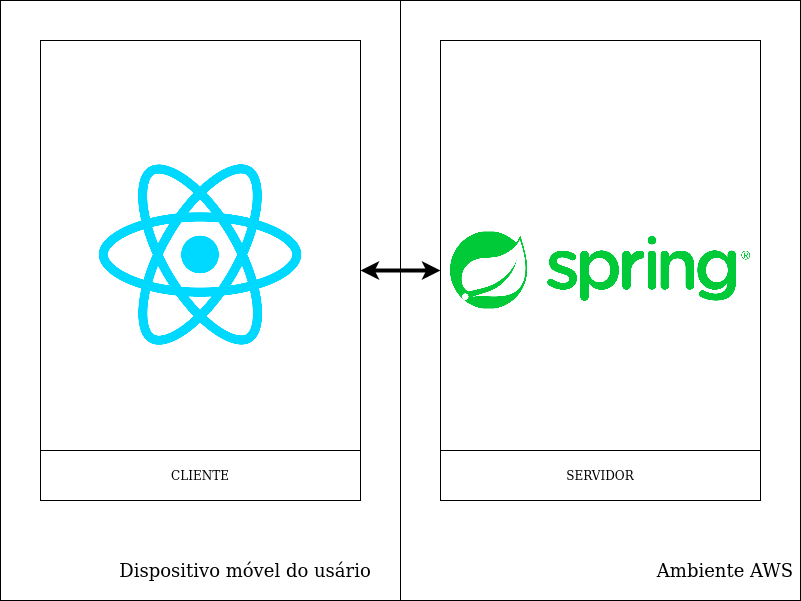
\includegraphics[scale=0.4]{lixt}
\end{figure}

A comunicação entre estes serviços será feita com o uso do protocolo
\label{sig:https}\hyperlink{s:http}{HTTPS}, que permite a aplicação
cliente realizar chamadas ao servidor através de urls, seja para
buscar informações para apresentar ao usuário ou postar informações
coletadas dele. O \gls{framework} Spring, além de abstrair a implementação
da lógica de um servidor, implementa \emph{listeners} para estas urls,
auxiliando a criação de pontos na aplicação do servidor focados na
comunicação com a aplicação cliente.

O uso do protocolo HTTPS oferece alguamas vantagens a aplicação
\gls{frontend}, que não precisa esperar uma solicitação ao
\gls{backend} ser finalizada antes de realizar outras solicitações,
aumentando a repsonsividade da aplicação cliente. Para além disso,
quando combinada ao modelo \label{sig:rest}\gls{REST} na
construção da \label{sig:API}\gls{API}, o protocolo HTTP
oferece meios eficientes para que as aplicações se comuniquem.

Como plataforma de servidor, o serviço AWS será utilizado, uma vez que
é oferecida de maneira gratuita para a realização deste projeto, e nele
serão armazenadas algumas instâncias da aplicação \gls{backend}.
Esta redundância é necessária como forma de garantir a estabilidade do
sistema, de forma que sempre haja alguma disponível para o
processamento de novas requisições, e, em caso de falha numa delas, o
serviço não seja interrompido aos usuários.

%%% Local Variables:
%%% mode: latex
%%% TeX-master: "../../desenho"
%%% End:


\section{Escopo do Projeto}

Lixt é um aplicativo para gerenciamento de listas de compras compartilhadas ou não.

O aplicativo vai seguir a dinâmica de uso abaixo:
\begin{enumerate}
	\item O usuário cria uma lista de compras e insere todos os itens antes da compra;
	\item O usuário inicia um carrinho de compras quando chega ao mercado, nesse momento ele tem a opção de importar para aquele carrinho os itens das listas que ele possui em aberto (que ainda não foram finalizadas), marcando quais listas ele deseja que sejam incluídas. Com o carrinho de compras ele poderá anotar os preços dos itens, riscá-los e ver o total gasto. Ao finalizar a compra as listas são atualizadas, e já aparecem riscados os itens que já foram comprados;
	\item Quando o usuário definir que uma lista não é mais relevante ele poderá deletar a lista ou desmarcar todos os itens, para reutilizar a lista.
\end{enumerate}

A seguir listamos as principais funcionalidades como uma lista de tópicos para facilitar a visualização de quais funcionalidades dependem de outras de forma hierárquica:

\begin{itemize}
	\item \textit{Login}:
		\begin{itemize}
			\item Criar conta;
			\item Redefinir senha;
		\end{itemize}
	\item Editar uma lista:
		\begin{itemize}
			\item Adicionar item:
				\begin{itemize}
					\item Definir nome;
					\item Definir quantidade;
					\item Definir unidade de medida (un. ml, L etc.);
					\item Definir medida;
					\item Adicionar uma categoria:
						\begin{itemize}
							\item Criar nova categoria;
						\end{itemize}
					\item Adicionar um comentário;
					\item Atribuir a um usuário (caso a lista tenha sido compartilhada e pelo menos um convite já tenha sido aceito);
				\end{itemize}
			\item Remover itens;
			\item Convidar pessoas para a lista (apenas quem criou a lista):
				\begin{itemize}
					\item Enviar convite:
						\begin{itemize}
							\item Acompanhar \textit{status} (aceito ou pendente);
							\item Remover convite;
						\end{itemize}
				\end{itemize}
			\item Deletar uma lista;
			\item Limpar uma lista;
		\end{itemize}
	\item Iniciar um carrinho de compras:
		\begin{itemize}
			\item Selecionar listas para compor o carrinho;
			\item Informar o mercado onde a compra será realizada (automaticamente através da localização, se não estiver habilitada será solicitado que o usuário insira o nome do mercado);
			\item Exibir o valor total do carrinho;
			\item Informar a quantidade que será efetivamente comprada naquele momento (o usuário pode ter planejado 10 unidades e apenas comprar 5 naquele momento);
			\item Riscar itens;
			\item Finalizar um carrinho de compras;
		\end{itemize}
	\item Ver estatísticas:
		\begin{itemize}
			\item Selecionar uma lista e ver o total gasto naquela lista ao longo do tempo em um gráfico de linha:
				\begin{itemize}
					\item Selecionar um dos pontos do gráfico e ver detalhes daquela lista;
				\end{itemize}
			\item Selecionar uma lista para ver um gráfico de pizza com os valores médios gastos por categorias naquela lista;
			\item Verificar histórico de preços de um item (tabela com nome do produto, quantidade, marca, preço, mercado e data da compra):
				\begin{itemize}
					\item Selecionar uma lista, dentro da lista selecionada selecionar o produto para ver o histórico;
				\end{itemize}
		\end{itemize}
\end{itemize}

Para o \textit{Minimum Viable Product} (\label{sig:mvp}\hyperlink{s:mvp}{MVP}) vamos implementar as seguintes funcionalidades, as demais ficarão para o próximo semestre:

\begin{itemize}
	\item \textit{Login}:
		\begin{itemize}
			\item Criar conta;
			\item Redefinir senha;
		\end{itemize}
	\item Criar lista de compra:
		\begin{itemize}
			\item Atribuir um nome;
			\item Atribuir uma descrição;
			\item Importar uma lista anterior;
		\end{itemize}
	\item Editar uma lista:
		\begin{itemize}
			\item Adicionar item:
				\begin{itemize}
					\item Definir nome;
					\item Definir quantidade;
					\item Definir unidade de medida (un., ml., L etc);
					\item Definir medida;
					\item Adicionar a uma categoria:
						\begin{itemize}
							\item Criar uma nova categoria;
						\end{itemize}
					\item Adicionar um comentário;
					\item Atribuir a um usuário (caso a lista tenha sido compartilhada e pelo menos um convite já tenha sido aceito);
				\end{itemize}
			\item Remover itens;
			\item Convidar pessoas para a lista (apenas quem criou a lista):
				\begin{itemize}
					\item Enviar convite:
						\begin{itemize}
							\item Acompanhar  status (aceito ou pendente);
							\item Remover convite;
						\end{itemize}
				\end{itemize}
			\item Deletar uma lista;
			\item Limpar uma lista;
		\end{itemize}
	\item Iniciar um carrinho de compras:
		\begin{itemize}
			\item Selecionar listas para compor o carrinho;
			\item Informar o mercado onde a compra será realizada (será solicitado que o usuário insira o nome do mercado manualmente);
			\item Exibir o valor total do carrinho;
			\item Informar a quantidade que será efetivamente comprada naquele momento (o usuário pode ter planejado 10 unidades e apenas comprar 5 naquele momento);
			\item Riscar itens;
			\item Finalizar o carrinho de compras.
		\end{itemize}
\end{itemize}

\subsubsection{Requisitos Funcionais}

Os requisitos funcionais dizem respeito às funcionalidade que o sistema deve ter. O Quadro \ref{reqFuncionais} lista os requisitos funcionais, suas dependências, a sigla e a prioridade de implementação.

\begin{quadro}[H]
\caption{Requisitos funcionais}
\begin{tabular}{|l|l|l|l|l}
\cline{1-4}
\textbf{Sigla} & \textbf{Descrição}                                                                                                                                                                                                                                               & \textbf{Prioridade} & \textbf{Dependências} &  \\ \cline{1-4}
RF01           & \begin{tabular}[c]{@{}l@{}}\textit{Login}: o usuário deve ser capaz de criar \\ sua conta no aplicativo, definir sua senha e \\ realizar o \textit{login} no sistema.\end{tabular}                                                                                                 & Alta                &                       &  \\ \cline{1-4}
RF02           & \begin{tabular}[c]{@{}l@{}}O sistema deve possibilitar que o usuário \\ crie suas listas de compras e possa atribuir um\\ nome, uma descrição e ter a opção de importar \\ uma lista existente.\end{tabular}                                                     & Alta                & RF01                  &  \\ \cline{1-4}
RF03           & \begin{tabular}[c]{@{}l@{}}Editar uma lista: Possibilita ao usuário o \\ gerenciamento dos itens da lista, como adicionar \\ itens, remover e enviar convites para a lista.\end{tabular}                                                                         & Alta                & RF02                  &  \\ \cline{1-4}
RF04           & \begin{tabular}[c]{@{}l@{}}Iniciar um carrinho de compras: permitir que o \\ usuário importe várias listas de compras, informe \\ o local da compra, o total gasto, quantidade de \\ itens a ser comprados, riscar itens e finalizar \\ o carrinho.\end{tabular} & Alta                & RF03                  &  \\ \cline{1-4}
RF05           & \begin{tabular}[c]{@{}l@{}}Ver estatísticas: ver o histórico de valores \\ pagos em uma lista ao longo do tempo, ver \\ os valores gastos por categorias em uma lista, \\ ver o histórico de preços de um determinado \\ item ao longo do tempo.\end{tabular}    & Média               & RF04                  &  \\ \cline{1-4}
\end{tabular}
\fonte{Os Autores}
\label{reqFuncionais}
\end{quadro}


\subsubsection{Requisitos Não Funcionais}

De maneira simplificada, os requisitos não funcionais não estão relacionados diretamente às funcionalidades do sistema, mas ao seu funcionamento de um modo geral, ou seja, como ele as funcionalidade serão executadas.

No Quadro \ref{reqNaoFuncionais} estão elencados os requisitos não funcionais, cada um com sua nomenclatura, categoria e descrição.

\begin{quadro}[H]
\caption{Requisitos Não funcionais}
\begin{tabular}{llll}
\cline{1-3}
\multicolumn{1}{|l|}{\textbf{Nomenclatura}} & \multicolumn{1}{l|}{\textbf{Descrição}}                                                                                                                                                                                                            & \multicolumn{1}{l|}{\textbf{Categoria}} &  \\ \cline{1-3}
\multicolumn{1}{|l|}{RNF01}                 & \multicolumn{1}{l|}{\begin{tabular}[c]{@{}l@{}}Criptografia das senhas: Por uma questão \\ de segurança as senhas não serão \\ armazenadas diretamente no banco, serão \\ criptografadas antes de serem armazenadas \\ como um \textit{hash}.\end{tabular}} & \multicolumn{1}{l|}{Segurança}          &  \\ \cline{1-3}
\multicolumn{1}{|l|}{RNF02}                 & \multicolumn{1}{l|}{\begin{tabular}[c]{@{}l@{}}Comunicação: A comunicação entre as \\ camadas da aplicação deverá ser feita utilizando \\ o protocolo HTTPS, para garantir a segurança \\ no envio dos dados através da rede.\end{tabular}}        & \multicolumn{1}{l|}{Segurança}          &  \\ \cline{1-3}
\multicolumn{1}{|l|}{RNF03}                 & \multicolumn{1}{l|}{\begin{tabular}[c]{@{}l@{}}Responsividade: O sistema deve exibir \\ corretamente os elementos da interface gráfica \\ nos mais variados tamanhos de celulares.\end{tabular}}                                                   & \multicolumn{1}{l|}{Usabilidade}        &  \\ \cline{1-3}
\multicolumn{1}{|l|}{RNF04}                 & \multicolumn{1}{l|}{\begin{tabular}[c]{@{}l@{}}Internacionalização: O sistema deverá suportar \\ dois idiomas (inglês e português) e suportar \\ que futuramente seja possível adicionar outros \\ idiomas.\end{tabular}}                          & \multicolumn{1}{l|}{Usabilidade}        &  \\ \cline{1-3}
\multicolumn{1}{|l|}{RNF05}                 & \multicolumn{1}{l|}{\begin{tabular}[c]{@{}l@{}}Escalabilidade: O sistema deverá ser projetado \\ para garantir que futuras melhoras e expansões \\ sejam possíveis.\end{tabular}}                                                                  & \multicolumn{1}{l|}{Desempenho}         &  \\ \cline{1-3}
\multicolumn{1}{|l|}{RNF06}                 & \multicolumn{1}{l|}{\begin{tabular}[c]{@{}l@{}}Disponibilidade: O sistema deverá estar disponível \\ aos usuários ininterruptamente\end{tabular}}                                                                                                  & \multicolumn{1}{l|}{Disponibilidade}    &  \\ \cline{1-3}
                                            &                                                                                                                                                                                                                                                    &                                         & 
\end{tabular}
\label{reqNaoFuncionais}
\fonte{Os Autores}
\end{quadro}

\section{Tecnologias Utilizadas}

As tecnologias que decidimos utilizar foram escolhidas a partir do conhecimento prévio da equipe, da curva de aprendizado e levando em consideração também o tamanho das comunidades que já a utilizam, visando um maior apoio e material de pesquisa.
Dito isso, escolhemos as seguintes tecnologias:

\subsection{Linguagens}

\subsubsection{Back-end}

Decidimos que a linguagem para o \gls{backend} seria o Java. A linguagem se adequa à nossa proposta e atende o paradigma de linguagem orientada a objetos do qual nos foi orientado a utilizar. 
A comunidade de Java é extensa e ativa, contribuindo com muitos materiais e recursos. Ainda podemos destacar que a utilização da linguagem previamente pelos integrantes da equipe também foi impactante na consolidação dessa decisão.

\subsubsection{Mobile}
Para o desenvolvimento da plataforma mobile decidimos utilizar o Javascript. A linguagem possui também uma comunidade ativa e uma variedade de materiais disponíveis e atualizados. Apesar de nem todos os integrantes terem tido contato prévio, por conta da facilidade de assimilação e necessidade de poucos recursos para a configuração do ambiente de desenvolvimento, optamos pelo Javascript.

\subsection{Frameworks e ORMs}

\subsubsection{Back-end}

Para o \gls{backend} decidimos utilizar o \gls{framework} Spring, usando a ferramenta Spring Boot que proporciona agilidade na criação das aplicações pois segue a filosofia de Convention over Configuration\cite{Devopedia2020}, nos poupando de depreender muito tempo nas configurações. Não obstante, a \gls{framework} facilita o desenvolvimento pois nos propicia a utilização de módulos que julgarmos necessários (como Spring MVC e Spring Data JDBC). Além disso, há uma gama vasta de materiais para consultarmos.
Como ferramenta \gls{ORM} decidimos usar o Hibernate pela consolidação dele no mercado e o uso amplo em aplicações Java que necessitam de mapeamento relacional dos dados. Por conta da quantidade de modelos da aplicação, julgamos necessário utilizar uma ferramenta que facilitasse esse processo. 

\subsubsection{Mobile}
Na aplicação mobile decidimos utilizar o \gls{framework} React-Native. Esta \gls{framework} gera aplicativos nativos, não necessita de muitos recursos e configurações para montar o ambiente de desenvolvimento e possibilita um conforto maior no desenvolvimento do código por ser uma \gls{framework} Javascript. Não obstante, também é uma \gls{framework} com larga quantidade de recursos para consulta além de uma comunidade muito ativa.

\subsection{Banco de dados}
O banco de dados que escolhemos foi o MySQL pois precisávamos para a nossa proposta de um banco de dados relacional e que fosse possível de ser hospedado na AWS. Verificamos que o MySQL cobria não apenas esses critérios mas também possui uma ferramenta gráfica (MySQL Workbench) que facilita a visualização e a operação do banco. Além disso os integrantes da equipe já tiveram experiências com a ferramenta anteriormente.

\subsection{Gerenciamento de tarefas}
Para o gerenciamento das tarefas optamos pela ferramenta Trello por ser gratuita, de fácil manuseio e visualização.
Além disso, o Trello figura entre as ferramentas que foram utilizadas com sucesso nos semestres anteriores durante o desenvolvimento de projetos.

\subsection{Versionamento}
Para o controle de versão do desenvolvimento da aplicação optamos pelo Git com repositório no Github. Esta escolha foi realizada devido à experiência prévia da equipe com a ferramenta e pela quantidade de recursos oferecidos pela plataforma na gestão do desenvolvimento de aplicações.
Para o versionamento do projeto utilizamos o Apache Subversion (SVN). Concentramos no repositório fornecido pelos professores todas as entregas previstas (incluindo as versões atualizadas dos códigos do repositório externo do Github).



%%% Local Variables:
%%% mode: latex
%%% TeX-master: "../proposta"
%%% End:


\section{Escalabilidade}

A escalabilidade da aplicação é sua capacidade de se adequar a um
amplo volume de requisições, mantendo a estabilidade do sistema e a
velocidade de respostas. Um sistema escalável está apto para responder
adequadamente nestes momentos, assim como liberar seus recursos em
momentos com poucas requisições.

Por se tratar de algo relativo ao processamento de requisições, a
escalabilidade diz respeito ao \gls{backend}, que centraliza os
pedidos dos usúarios. A camada cliente por outro lado, por focar
exclusivamente na lógica de visualização, e rodar em dispositivos
mobile, não exige tanta capacidade de processamento, e a
escalabilidade não é uma preocupação para esta camada.

Como foi mencionado, a aplicação \gls{backend} ficará armazenada na
plataforma Amazon AWS. Existe um processo da ferramenta de integração
contínua Jenkins para aumentar o número de instâncias ativas em
produção, e este processo será acionado em momentos com intenso volume
de requisições.


%%% Local Variables:
%%% mode: latex
%%% TeX-master: "../../desenho"
%%% End:


\section{Manutenibilidade da aplicação}

É fundamental para o desenvolvimento do projeto, tanto o previsto
quanto em avanços posteriores, que a aplicação atinja um nível adequado
de qualidade, e para tanto certos requisitos de manutenibilidade devem
ser estabelecidos.  Estes requisitos permitem estabelecer critérios
para medir o quanto o processo de desnvolvimento está de acordo com
boas práticas, e incentivam que estas práticas sejam seguidas.

\subsection{\emph{Logs}}

Como forma de monitorar a aplicação em tempo de execução,
especialmente na camada de servidor, \emph{logs} serão usados para
registrar o estado dos objetos. A ferramenta Log4j será usada, uma vez
que os membros da equipe já tem mais familiaridade com ela. Esta
ferramenta perimite o registro em diversos níveis, como
\begin{itemize}
  \em
\item info
\item debug
\item warn
\item error
\end{itemize}
e pode ser configurada para que apenas os dois últimos
sejam registrados no ambiente de produção. Desta forma a cada ponto de
falha da aplicação um log de nível apropriado será colocado para que
problemas sejam rapidamente identificados, analisados e resolvidos.

\subsection{Integração Contínua}

Visando manter o serviço sempre atualizado para o usuário, a
ferramenta de integração contínua Jenkins foi selecionada para a
implantação da aplicação \gls{backend} em produção. Ela permite a
configuração de tarefas, também chamada de \emph{jobs}, que facilitam
a implantação do sistema.

O diagrama \ref{fig:jenkins} ilustra o funcionamento da ferramenta:
\begin{enumerate}
\item uma instância dela, rodando no ambiente AWS tem acesso ao código no
github;
\item no momento do \gls{deploy}, a instância, rodando em uma máquina
  virtual cria um processo filho, que realiza o \emph{checkout} do
  código fonte no Github, executa testes e o \emph{build} da
  aplicação;
\item uma cópia deste \emph{build} é salva em uma máquina virtual
  secundária, como histórico das versões da aplicação;
\item pr fim, na máquina virtual final, onde o sistema será
  implantado, a imagem é copiada e iniciada.
\end{enumerate}
Vale notar que, quando o \emph{deploy} é realizado, uma instância só é
derrubada quando uma nova instância, de uma nova versão, está
plenamente operante.

\begin{figure}
  \centering
  \caption{Diagrama ilustrando o processo de \emph{deploy}.}
  \includegraphics[scale=0.50]{images/deploy}
  \label{fig:jenkins}
\end{figure}

Para o \gls{frontend}, no entanto, não existem ferramentas de
integração contínua, uma vez que as imagens do aplicativo mobile
precisam ser aprovadas pelas lojas de aplicativo. Contudo, ainda é
possível usar ferramentas de CI para a execução de testes e
verificação da integridade do código a cada nova versão.

\subsection{\emph{Code Conventions}}

As convenções de código são acordos internos ao equipe que visam
estandartizar a forma como os diversos integrantes do equipe produzem
seus códigos.  Elas visam facilitar o entendimento mútuo entre os
integrantes da equipe, de modo o estilo de progamação seja indistiguível
e independente de seus autores.  Geralmente, as convenções de código
estabelecem estilos para se organizar o código textualmente, isto é,
dizem respeito a forma como nomes de variáveis são escolhidas e
comentários são posicionados, por exemplo.

As convenções adotadas são baseadas na especificação da
\citeauthor{Oracle1997}, de 1997. Esta é comumente usadas para o
desenvolvimento na linguagem Java, e muito próxima do padrão adotado
em JavaScript, e vale destacar o seguintes pontos:
\begin{itemize}
\item Minimizar o uso de variáveis, funções e objetos globais.
\item As declarações globais estarão preferencialmente no início do arquivo.
\item Declarar as variáveis próximo do ponto onde elas serão inicializadas.
\item A indentação é de 4 espaços.
\item Linhas mais longas que 80 caracteres serão quebradas e
  indentadas a 8 espaços.
\item Pacotes e variáveis com nomes curtos, em \texttt{camelCase} e substantivos.
\item Classes e interfaces em \texttt{CamelCase} e substantivos.
\item Métodos em \texttt{camelCase} e verbos.
\item Constantes em \texttt{UPPER\_CASE}.
\end{itemize}

No entanto, especificamente para a linguagem Java,
\begin{itemize}
\item Classes e métodos devem ser documentados com um comentário na
  seguinte forma, uma vez que as IDEs reconhecem este formato e
  formatam o text na forma de \emph{pop-ups} quando o cursor está
  sobre uma referência a esta classe.
\begin{verbatim}
/**
 * Class ListService
 *
 * Implementar endpoints para as funcionalidades de lista.
 */
\end{verbatim}
\end{itemize}

No backend, a estrutura de pacotes vai ser bem dividida, tendo o pacote controller para os controllers e endpoints, mapper para os mappers. O model, service e repository de uma entidade ficarão no mesmo pacote cujo nome é o mesmo nome da entidade.

\subsection{\emph{Designs Patterns}}

Como padrões de projetos, serão usados 3 padrões amplamente utilizados pela comunidade de desenvolvimento: (I) Clean Code, (II) SOLID e (III) Gang Of Four. Esses 3 padrões podem ser utilizados tanto no backend quanto no frontend.

\subsubsection{\emph{Clean Code}}

O Clean Code é um conjunto de boas práticas para melhorar o entendimento do código, de modo que seja mais fácil sua leitura. Segue abaixo uma lista das principais boas práticas:

\begin{itemize}
	\item Nome Significativos para variáveis, classes, métodos, atributos e objetos, evitando abreviaturas desnecessárias e nomes não recorrentemente utilizados, sendo passíveis de busca.
	\item Evitar números mágicos, recomendando-se utilizar enums e constantes para que seja mais compreensível ao analisar o código.
	\item Evitar booleanos de forma implícita.
	\item Evitar condicionais negativos (por exemplo, uma função com nome "naoDevoExecutar()"), visto que dificulta a compreensão de código.
	\item Encapsular condicionais.
	\item Nunca comentar o óbio no código.
	\item Utilizar funções pequenas, tanto para melhorar a leitura quanto para respeitar os padrões do SOLID.
\end{itemize}

\subsubsection{\emph{SOLID}}

O SOLID é um acrônimo de 5 príncipios da Programação Orientada a Objetos, sendo fundamental para o desenvolvimento e manutenção de software.

\begin{itemize}
	\item \underline{\textbf{S}ingle Responsiblity Principle}: Uma classe deve ter apenas um motivo para mudar.
	\item \underline{\textbf{O}pen-Closed Principle}: Uma classe deve estar aberta para extensão, e fechada para modificação, recomendando sempre utilizar a herança e não modificar o código fonte original.
	\item \underline{\textbf{L}iskov Substitution Principle}: Uma classe derivada deve ser substituível por sua classe base.
	\item \underline{\textbf{I}nterface Segregation Principle}: Utilizar muitas interfaces específicas é melhor do que uma interface genérica.
	\item \underline{\textbf{D}ependency Inversion Principle}: Dependa de abstrações e não de implementações.
\end{itemize}

\subsubsection{\emph{Gang Of Four}}

O GoF (ou Gang of Four) se refere aos profissionais que criaram os 23 padrões de projetos, nos quais seus conceitos serão utilizados no desenvolvimento do Lixt.

Segue abaixo uma breve apresentação dos principais padrões utilizados:

\begin{itemize}
	\item \underline{Builder}: Será utilizado para criar instâncias legíveis de objetos complexos.
	\item \underline{Facade}: Encapsula regras de negócios complexas.
	\item \underline{Observer}: Observa e é capaz de reagir às mudanças de estado de um objeto.
\end{itemize}

\subsection{Testes}

Testes são uma ferramenta fundamental para o desenvolvimento da
aplicação, uma vez que garantem, em tempo de compilação, o
comportamento correto do aplicativo. Para além disso, testes tem um
papel de documentação, uma vez que encapsulam de forma breve o
comportamento esperado das classes e métodos produzidos, e podem ser
consultados em caso de dúvida quando ao uso destes. Este tipo de teste
é chamado de teste unitário, em oposição aos testes de integração, que
verificam o funcionamento da aplicação de ponta-a-ponta, isto é, a
partir de uma chamada a um endpoint, apenas os serviços externos são
mimetizados, garantindo o funcionamento correto de toda a aplicação.

Desta forma, a construção de testes, de ambos os tipos é de extrema
importância para a elaboração do projeto visando a sua
manutenibilidade, e será o primeiro passo de uma sprint, após o
planejamento, a construção de testes relevantes para a tarefa,
seguindo os princípios do TDD\cite{TDD}. Como as ferramentas de teste são
específicas de cada linguagem, cada camada da aplicação fará uso de
frameworks distintos.

O \gls{backend} será testado com o framework JUnit, fazendo uso da
biblioteca Mockito quando necessário simular comportamentos de objetos
que não são o alvo da suite de teste. Este framework ainda oferece
ferramentas para testar o banco de dados, ou melhor, testar a conexão
com o banco e verificar o comportamento das classes de acesso a ele.
Já os teste de \gls{frontend} serão feitos com a biblioteca Jest,
que auxilia a construção de testes unitários, e por se tratar de uma
\gls{GUI}, as interações de usuário devem ser simuladas também. Para tanto, a
biblioteca React Testing Library será usada.

%%% Local Variables:
%%% mode: latex
%%% TeX-master: "../../desenho"
%%% End:


\input{capitulos-desenvolvimento/section/segurança}

\section{Viabilidade Financeira}

O projeto de análise de viabilidade financeira consiste em averiguar a garantia de lucro sobre as despesas do projeto. Portanto, nesse projeto será descrito cada processo a fim de fazer essa verificação.

\subsection{Gerenciamento de Custos}

Nesse tópico, serão abordados temas de investimento inicial e de desenvolvimento do projeto, incluindo tópicos de análise de requisitos, desenvolvimento, manutenções e imprevistos.

\subsubsection{Análise de Requisitos e Desenvolvimento}

Para iniciar o projeto, é necessário fazer os primeiros planejamentos, elicitação de requisitos, abstrair e concretizar as primeiras ideias e fazer os primeiros planejamentos (diagramas, cronogramas e documentação). Logo após, o projeto chega na fase de desenvolvimento, onde é começado a se tornar real.

Contudo, o projeto não vai possuir nenhum custo de análise e implementação do sistema, devido ao fato de ser um projeto educacional.

\subsubsection{Manutenções}

Inevitavelmente, manutenções do sistema ocorrerão pós finalização do projeto e estar devidamente funcional em produção. Contudo, os custos de manutenções também não serão cobrados, devido a ser um projeto educacional.

\subsection{Custos de deploy e de Ambiente de Produção}

Nesse tópico, são apresentados os custos de manter o sistema funcional e disponível para os usuários. Desse modo, será feito uma previsão anual de cada plataforma utilizada:

\subsubsection{Frontend} 

Tendo em vista que o projeto é \textit{mobile} voltado para dispositivos Android, será publicado na PlayStore, estimando um valor de 25.00 USD anual. 

\subsubsection{Backend}

Inicialmente gratuito no Amazon EC2, sendo permitido 750h de instâncias por mês durante o período de 12 meses.

A partir do momento que for necessário grande porte, será indicado o plano Sob Demanda do Amazon EC2, que garante viabilidade econômica e estratégica (visto que o preço é calculado a partir do uso). 

Utilizando a calculadora da AWS e optando por um servidor Linux da instância t4g.micro com 1 vCPU e 1GiB, com armazenamento SSD de uso geral de 10GB, será custeado o valor de 7,52 USD mensalmente para operar o mês inteiro.

\subsubsection{Banco de Dados} 

Inicialmente gratuito no Amazon RDS, sendo permitido 750h de instâncias durante o período de 12 meses. O Amazon RDS possui suporte a vários \gls{sgbd}, incluindo o MySQL, que foi o \gls{sgbd} optado para desenvolver a aplicação Lixt.

A partir do momento que for necessário grande porte, será indicado o plano Sob Demanda do Amazon RDS, que garante viabilidade econômica e estratégica (visto que o preço é calculado a partir do uso).

Utilizando a calculadora da AWS e optando por um servidor da instância t2.micro de modelo Single-AZ OnDemand, com armazenamento SSD para cada instância de 10GB, será custeado o valor de 27,74 USD mensalmente para operar o mês inteiro.

\subsection{Medidas de Obtenção de Retorno Financeiro}

Para gerar uma receita positiva a fim de obter lucro, haverá duas formas principais de retorno financeiro:

\begin{itemize}
	\item \underline{Cobrança do aplicativo}: O aplicativo estará disponível gratuitamente na PlayStore, não gerando, portanto, retorno financeiro.
	\item \underline{Propaganda/Recomendação}: Será utilizado mediador de anúncio AdMob (responsável por conectar aplicações e anunciantes), onde o valor varia por visualizações de anúncios e cliques neles. Contudo, no próprio site do admob, é citado um caso no qual houve 300.000 downloads e arrecadava, através do AdMob, 100 USD por dia. \cite{GoogleAdMob}
\end{itemize}

A partir da calculadora do AdMob, estimando-se uma quantidade de 250 visitantes por dia, onde há 2 paginas visualizadas por visitante, sendo que a taxa de cliques em anúncios é 1\% e o custo do clique é 0.35 USD, o valor mensal será de 52.5 USD.

\subsection{Conclusão}

Concluindo que, ao utilizar os servidores de baixo porte detalhados acima, será desembolsado cerca de 35.00 USD por mês. Contudo, o valor calculador para 250 visitantes (estimando o valor com baixo engajamento) com os parâmetros detalhados arrecadará 52.5 USD, conseguindo custear os servidores e ainda garantindo margens de lucro.

Conforme o engajamento na aplicação for aumentando, será revisto os planos dos servidores para atender maiores níveis de requisições.


%%% Local Variables:
%%% mode: latex
%%% TeX-master: "../desenho"
%%% End:

\chapter{Planejamento e Gerenciamento do Projeto}
As próximas seções possuem o objetivo de descrever mais sobre como a equipe e o projeto estão organizados quanto a metodologia, papéis de atuação, gestão de tempo e divisão de tarefas.

\section{Metodologia de Gestão e Desenvolvimento de Projeto}
O grupo optou pelo uso de uma metodologia ágil para o projeto e, após
algumas reuniões, foi decidido que o que guiaria o processo de
desenvolvimento seria uma junção de frameworks extremamente úteis para
a melhor performance do time, o \gls{scrum} e o \gls{kanban}.  O \gls{scrum}
se baseia na divisão do projeto em vários ciclos de atividades ---
conhecidos como sprints - com diversas cerimônias e interações
frequentes da equipe a fim de alinhar o que tem sido feito, tratar
impedimentos e pensar em maneiras de otimizar o processo de trabalho,
aumentando a agilidade no desenvolvimento. Já o \gls{kanban} é um
método de controle e gestão de forma visual, geralmente feito com o
uso de post-its coloridos que reforçam a simbologia das tarefas e
ações que precisam ser feitas, estão sendo feitas, ou foram
concluídas.

Dentro das metodologias ágeis é muito comum - e essencial - a
definição do \gls{product-backlog} contendo todas as funcionalidades
desejadas na aplicação pelo cliente e elencadas por prioridade. Esse
backlog é, posteriormente, dividido em tarefas que serão distribuídas
em cada Sprint, gerando o \gls{sprint-backlog}. É nesse momento em que, no
projeto, o Kanban será aplicado. Dessa forma, o \gls{scrum} será utilizado
para a determinação do método de desenvolvimento iterativo e
incremental e o \gls{kanban} será utilizado para métricas e fluxos de
produção da equipe.

\section{Organização da Equipe}
As primeiras reuniões de alinhamento entre os membros da equipe foram essenciais para que os integrantes pudessem interagir e compartilhar mais sobre quais conhecimentos prévios possuem, quais são suas áreas de maior facilidade e interesse e dessa forma planejar uma estratégia de desenvolvimento que, apesar de desafiadora, também seja inclusiva a todos do grupo. 

No Scrum, metodologia escolhida para o projeto, a definição de alguns papéis é necessária. São eles: 

\begin {itemize}
\item \textbf{Product Owner}: É o responsável pelos interesses do cliente no projeto, captando, interpretando e repassando ao time de desenvolvimento suas necessidades. Quem assumiu este papel foi o Fabio Mendes;

\item \textbf{Scrum Master}: É o facilitador no desenvolvimento do projeto, cuidando para que as cerimônias do Scrum sejam devidamente cumpridas e ajudando a resolver os impedimentos que possam atrapalhar a equipe de desenvolvimento. Quem assumiu este papel foi a Carolina de Moraes;

\item \textbf{Development Team}: Time que cuida do desenvolvimento técnico do projeto. Quem assumiu este papel foram Alkindar Rodrigues, Gabriely Bicigo, Leonardo Naoki e Mariana Zangrossi.

\end {itemize}

É importante salientar que, apesar da divisão de papéis, todos os participantes estão contribuindo no desenvolvimento com o objetivo de entregar o projeto na data estimada.

Para uma divisão mais organizada e formal de tarefas, foi montado um quadro de responsabilidades de cada integrante referente aos tópicos de desenvolvimento do projeto.

\begin{center}
  \begin{quadro}[H]
	\caption{Quadro de responsabilidades}\label{tab:tab_resp}
    \begin{tabular}{|l|c|c|c|c|c|c|}
      \hline
      \multicolumn{1}{|c|}{\textbf{Atividade}} & \textbf{Alkindar}     & \textbf{Carolina}     & \textbf{Fabio}        & \textbf{Gabriely}     & \textbf{Leonardo}     & \textbf{Mariana}      \\ \hline
      Back-End                                 & x                     & \multicolumn{1}{l|}{} & x                     & \multicolumn{1}{l|}{} & x                     & \multicolumn{1}{l|}{} \\ \hline
      Banco de dados                           & x                     & \multicolumn{1}{l|}{} & x                     & \multicolumn{1}{l|}{} & x                     & \multicolumn{1}{l|}{} \\ \hline
      Blog                                     & x                     & x                     & x                     & x                     & x                     & x                     \\ \hline
      Documentação                             & x                     & x                     & x                     & x                     & x                     & x                     \\ \hline
      Front-End                                & \multicolumn{1}{l|}{} & x                     & \multicolumn{1}{l|}{} & x                     & \multicolumn{1}{l|}{} & x                     \\ \hline
      Vídeos                                   & \multicolumn{1}{l|}{} & x                     & \multicolumn{1}{l|}{} & x                     & \multicolumn{1}{l|}{} & x                     \\ \hline
    \end{tabular}
		\fonte{Os Autores}
  \end{quadro}
\end{center}

%%% Local Variables:
%%% mode: latex
%%% TeX-master: "../../desenho"
%%% End:

\section{Gestão de Tempo}
Cada \gls{sprint} do projeto terá a duração de 2 semanas (10 dias úteis) e respeitará
todas as cerimônias do \gls{scrum}. Antes de dar início a uma nova sprint
ocorrerá a realização da \gls{planning}, reunião de planejamento onde
serão definidos os entregáveis da Sprint a ser iniciada. Após o início
da iteração, as dailies serão feitas através do grupo de mensagens
instantâneas do time. Ao fim do período de 2 semanas, ocorrerá a
\gls{review}, reunião com o objetivo de avaliar o que foi entregue
com sucesso naquela Sprint, e também a \gls{retrospective}, reunião
onde a equipe conversa sobre os pontos positivos e negativos da última
iteração e o que pode ser melhorado para a próxima Sprint. Todas essas
cerimônias foram incluídas no planejamento de gestão de tempo para o
cálculo da quantidade de Sprints necessárias até a entrega final do
projeto.

\begin{figure}[H]
  \centering
  \caption{Timeline do projeto}
  \label{fig:timelineProjeto}
  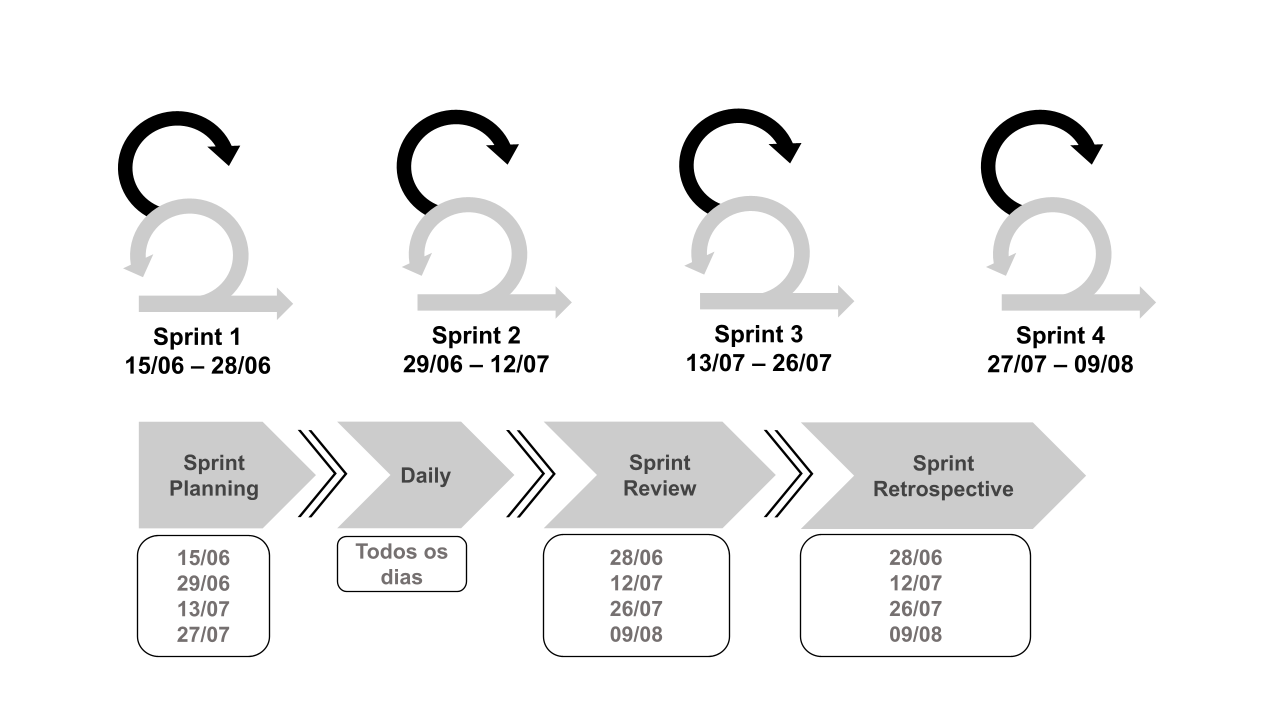
\includegraphics[scale=0.3]{Timeline}
	\fonte{Os Autores}
\end{figure}

%%% Local Variables:
%%% mode: latex
%%% TeX-master: "../../desenho"
%%% End:

\section{Histórias de usuário}
Para uma melhor estimativa e planejamento do projeto, histórias de usuário foram desenvolvidas para expressar funcionalidades do aplicativo que agreguem valor para seus usuários. Elas se originaram a partir das opiniões e sugestões de pessoas próximas que foram consultadas sobre o propósito do desenvolvimento, como familiares, amigos e principalmente os professores da disciplina. A tabela abaixo apresenta a descrição de todas as histórias de usuário geradas.

\begin{quadro}[H]
\caption{Histórias de usuário}
\resizebox{\textwidth}{!}{%
\begin{tabular}{|l|}
\hline
\multicolumn{1}{|c|}{\textbf{Histórias de usuário}}                                                                                           \\ \hline
Eu, como usuário, \\ gostaria de fazer cadastro no aplicativo de maneira básica e simples.                                                       \\ \hline
Eu, como usuário, \\ gostaria de fazer login utilizando e-mail e senha para que eu possa usar as funcionalidades do aplicativo.                  \\ \hline
Eu, como usuário, \\ gostaria de poder fazer reset de senha caso esqueça meu login.                                                              \\ \hline
Eu, como usuário, \\ gostaria de poder visualizar meus dados do aplicativo: e-mail, nome, senha.                                                 \\ \hline
Eu, como usuário, \\ gostaria de poder ver as pessoas que convidei para minhas listas, e gostaria de poder ver os convites que recebi.           \\ \hline
Eu, como usuário, \\ gostaria de poder ver minhas configurações de conta, como idioma e versão, por exemplo.                                     \\ \hline
Eu, como usuário, \\ gostaria de poder deslogar do aplicativo se necessário.                                                                     \\ \hline
Eu, como usuário, \\ gostaria de poder criar uma ou mais lista de compras.                                                                       \\ \hline
Eu, como usuário, \\ quero poder visualizar as listas que criei com um resumo de quantidade de itens e membros.                                  \\ \hline
Eu, como usuário, \\ quero poder visualizar os itens de uma lista que eu criei.                                                                  \\ \hline
Eu, como usuário, \\ quero poder compartilhar a lista que criei com outro membro.                                                                \\ \hline
Eu, como usuário, \\ quero poder visualizar as pessoas com quem compartilhei a lista.                                                            \\ \hline
Eu, como usuário, \\ quero poder remover um membro da minha lista.                                                                               \\ \hline
Eu, como usuário, \\ quero poder adicionar mais itens a minha lista.                                                                             \\ \hline
Eu, como usuário, \\ quero poder editar informações de um item na minha lista e adicionar comentários.                                           \\ \hline
Eu, como usuário, \\ quero poder adicionar um item caso não ache ele na lista de categorias.                                                     \\ \hline
Eu, como usuário, \\ quero poder adicionar um item a uma categoria através do código de barras.                                                  \\ \hline
Eu, como usuário, \\ quero poder iniciar uma compra no app para indicar que estou no mercado.                                                    \\ \hline
Eu, como usuário, \\ quando iniciar a compra, quero poder ver todos os itens, \\ de todas as listas, ou filtrar por apenas uma lista em específico. \\ \hline
Eu, como usuário, \\ quando iniciar a compra, quero poder ver o total gasto e salvar o que foi comprado.                                         \\ \hline
Eu, como usuário, \\ quero poder usar a mesma lista em várias compras.                                                                           \\ \hline
Eu, como usuário, \\ quero poder registrar o local onde a compra foi realizada.                                                                  \\ \hline
\end{tabular}%
}
\fonte{Os Autores}
\end{quadro}
                                                               

\section{Diagrama de Gantt}
Através das histórias de usuário geradas, foram extraídas atividades que compõem as funcionalidades desejadas. Com essas atividades, foi feito o diagrama de Gantt do projeto, onde as tarefas foram distribuídas de maneira visual entre as sprints do grupo, a fim de organizar o cronograma de desenvolvimento. 

\begin{figure}[H]
  \centering
  \caption{Diagrama de Gantt}
  \label{fig:cli-srv}
  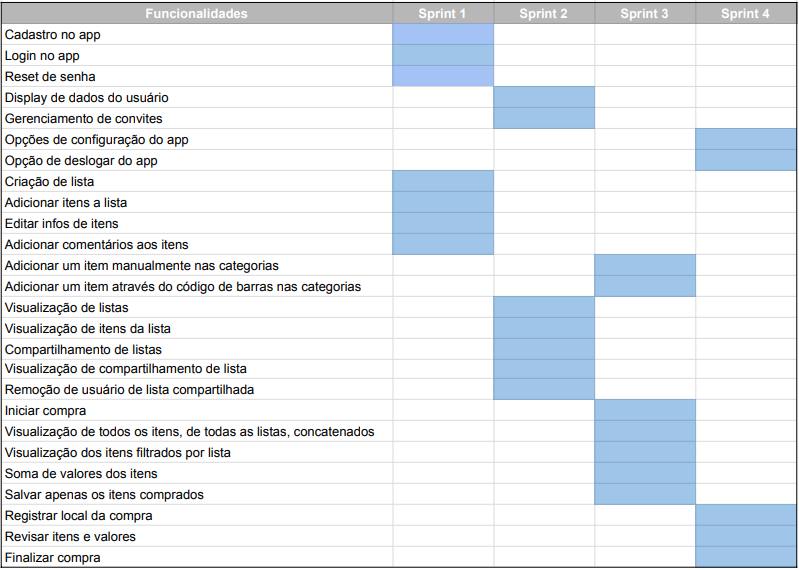
\includegraphics[scale=0.7]{Gantt}
	\fonte{Os Autores}
\end{figure}



% ----------------------------------------------------------
% Finaliza a parte no bookmark do PDF
% para que se inicie o bookmark na raiz
% e adiciona espaço de parte no Sumário
% ----------------------------------------------------------
\phantompart

% ----------------------------------------------------------
% ELEMENTOS PÓS-TEXTUAIS
% ----------------------------------------------------------
\postextual
% ----------------------------------------------------------

% ----------------------------------------------------------
% Referências bibliográficas
% ----------------------------------------------------------
% quando não esta utilizando biblatex tem que carregar as referencias aqui
\IfPackageLoaded{biblatex}{}{%
\bibliography{referencias}
}

% ----------------------------------------------------------
% Glossário
% ----------------------------------------------------------
%
%
\ifdef{\printnoidxglossary}{
\addcontentsline{toc}{chapter}{GLOSSÁRIO}
    \printnoidxglossary
    %\printglossaries
}{
 \chapter{GLOSSÁRIO}
 \printnoidxglossary
}


\end{document}